\newpage
\section{Morfeas ISO Channel Linker}
The ``Morfeas ISO Channel Linker" is an utility made to create ISO channels and link them with sensors.
It's can be accessed by the Morfeas WEB front page from the button with the anchor (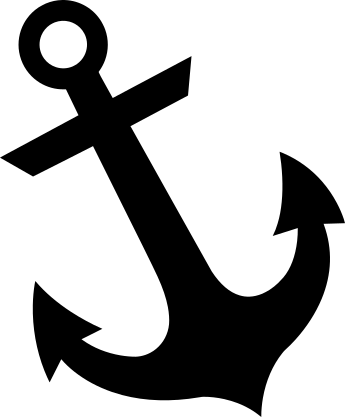
\includegraphics[height=.125in]{../art/anchor.png}).
At figure \ref{fig:ISOChannel_linker} shown an example of the ``Morfeas ISO Channel Linker" utility.

\begin{figure}[h]
\centering
	\fbox{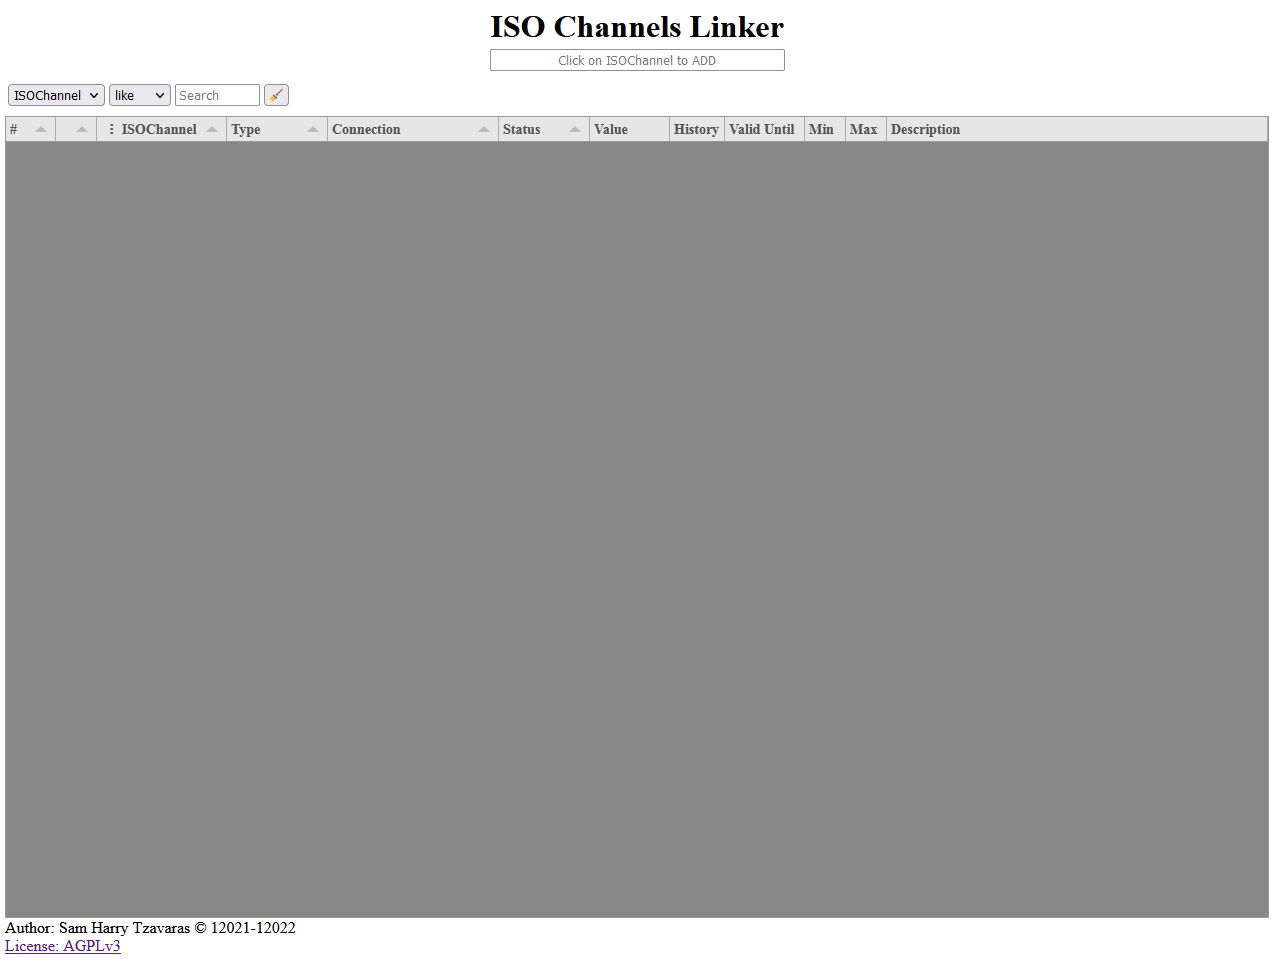
\includegraphics[width=3in,angle=0]{../art/Morfeas_web_if/Morfeas_WEB_ISOChannel_linker.png}}
	\caption{Morfeas ISO Channel Linker Utility}
	\label{fig:ISOChannel_linker}
\end{figure}
\noindent
The utility window split in three sections: the status bar, the filters section, and the ISO Channels table.\\

The status bar show the last update date if at least one channel exist,
or a message that informing the user to add channel(s).\\

The filter section, is filtering the ISO channels table, accordingly to the command from the user.
The filtering command is specified from the two drop-down lists and the text input field.
The first drop-down is selecting the column that the filtering will applied.
The second drop-down select the filter type; for most of the columns (except ``Min" and ``Max")
is ``like" and ``regex". The ``Like" filter type is filter and show all the elements in the specified column,
that contains the word in the search field, and similarly the ``regex" the fields that agree with the regular expression phrase.
For ``Min" and ``Max" the filter type change to a set of numerical comparing orders.
The button with the broom clean the filter.\\

The ISO Channels table is the configuration and presentation tool of the ``Morfeas ISO Channel Linker" utility.
It consist by 12 columns, with data for each ISO Channel.
The first column (from left) is show the order number of the ISO Channel.
The second column show with a color (table \ref{tab:col}) the status of each ISO Channel.
The third column contain the ISO Channel's name.
The forth and fifth contains the Connection type and path of the sensor that anchored to the ISO Channel.
Continue the sixth show the status of the anchored sensor, seventh the current value.
The eighth (History) contains a historical graph of past values of the sensors value, this graph show two minutes in past.
Next column show (if supported) the last valid date of the sensor.
The last three columns is the attributes of the ISO Channel; ``Min", ``Max" and ISO Channel's description.\\
Columns up to sixth can be shorted using the arrow at column name.
The shorting can be restored by clicking the filter clean button (broom).

\begin{table}[h!]
	\begin{center}
		\begin{tabular}{|c|l|}
			\hline
			\textbf{Color} & \textbf{Explanation}\\
			\hline
			Green & Okay\\
			\hline
			Orange & Calibration not valid\\
			\hline
			Red & Sensor warning\\
			\hline
			Black & OFF-Line/Disconnected\\
			\hline
		\end{tabular}
		\caption{Colors status}
		\label{tab:col}
	\end{center}
\end{table}

\subsection{Add new ISO Channel}
To add a new ISO Channel the ISOChannels menu can be used (figure \ref{fig:ISOCH_menu}) or the shortcut \textbf{Ctrl}+\textbf{Alt}+\textbf{A}.

\begin{figure}[h]
\centering
	\fbox{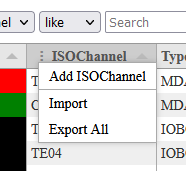
\includegraphics[width=2in,angle=0]{../art/Morfeas_web_if/Morfeas_WEB_ISOChannel_linker_menu.png}}
	\caption{ISOChannel's column menu}
	\label{fig:ISOCH_menu}
\end{figure}

By giving the ``Add ISOChannel" command (from menu or shortcut) a new window will appear (figure \ref{fig:ISOCH_new_link}).

\begin{figure}[h]
\centering
	\fbox{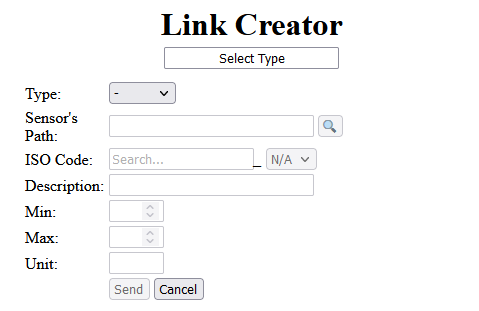
\includegraphics[width=3in,angle=0]{../art/Morfeas_web_if/Morfeas_WEB_ISOChannel_linker_link_creator.png}}
	\caption{ISO Channel Link Creator}
	\label{fig:ISOCH_new_link}
\end{figure}

